\documentclass[conference]{IEEEtran}

\usepackage[dvipdfmx]{graphicx}

\usepackage{bm}

\usepackage[fleqn]{amsmath}
\usepackage[psamsfonts]{amssymb}
\usepackage{url}

\newcommand{\birth}[1]{\mathcal{C}(#1)}
\newcommand{\distinct}[1]{\mathcal{N}_n^d(#1)}
\newcommand{\distinctnnn}[1]{\mathcal{N}_3^d(#1)}

\hyphenation{op-tical net-works semi-conduc-tor}

\begin{document}

\title{Identifying the Applied Obfuscation Method towards De-obfuscation}
% \title{Identified method of applied obfuscation for de-obfuscation}

% author names and affiliations
% use a multiple column layout for up to three different
% affiliations
\author{\IEEEauthorblockN{Hayato Sagisaka}
  \IEEEauthorblockA{Division of Frontier Informatics,\\
    Graduate School of Kyoto Sangyo University.\\
    Email: i1658065@cc.kyoto-su.ac.jp}
\and
\IEEEauthorblockN{Haruaki Tamada}
\IEEEauthorblockA{
  Faculty of Computer Science and Engineering,\\
  Kyoto Sangyo University\\
  Email: tamada@cc.kyoto-su.ac.jp}}

\maketitle

% As a general rule, do not put math, special symbols or citations
% in the abstract
\begin{abstract}
  Recently, to prevent cracking, the various protection methods have
  been proposed.  One of the protection methods is the obfuscation
  method. Obfuscation method changes the program to hard to understand
  in order to hide secret information in the program.
  %
  On the other hand, de-obfuscation is an interesting research topic
  for protecting the software.  Since, though vulnerable protection
  methods are dangerous, measuring the protection level was not
  discussed.
  %
  In this paper, we tackle to identify the applied obfuscation
  methods towards de-obfuscation.  To perform de-obfuscation requires
  a suitable method for each obfuscation method.  For this, we
  obfuscated programs by two practical tools and three algorithms
  from one academic tool.  Then, we analyzed the programs and
  extracted characteristics from them based on opcodes.  By using our
  method, we could identify the applied obfuscation method.

  % Recently, illegalities are increasing with the spread of software.
  % For the measures, there are methods of protect called obfuscation.
  % The obfuscation is method to do difficulty for analyzing to
  % program.  On the other hand, there is de-obfuscation that return
  % obfuscated program into former program.  De-change as different
  % method is to break the programs, it is necessary to identify that
  % obfuscation is applied to do de-obfuscation.  In this paper, we
  % measure find easy methods of protection by measuring to identify
  % easy method of protection.  Exactly, we analyze the obfuscated
  % programs and find the characteristic of obfuscation method.  Then,
  % we inspect that exacted characteristic is effective method for
  % unknown products and obfuscation methods.
\end{abstract}

% no keywords

% For peer review papers, you can put extra information on the cover
% page as needed:
% \ifCLASSOPTIONpeerreview
% \begin{center} \bfseries EDICS Category: 3-BBND \end{center}
% \fi
%
% For peerreview papers, this IEEEtran command inserts a page break and
% creates the second title. It will be ignored for other modes.
\IEEEpeerreviewmaketitle

\section{Introduction}
Recently, illegalities such as illegality access and analysis are
increasing.  Various methods of protection in software are proposed as
a measure.  Method of protection in software can guard from the
injustice access and analysis by prevent the program in advance.
There is a method of protection called obfuscation that is one of the
method of protection in software.  The obfuscation is method of
protection so as not to analyze program.
%
For example, name obfuscation that is to change unknown name of
meaning into class name and method name and control flow of
obfuscation that is to generate code that is not able to understand
the meaning when de-compile is tried to do are proposed various
methods how we falsify data so as not to analyze.  There are the
methods called de-obfuscation that is to return obfuscation program to
original program.  As de-obfuscation is taken by illegality access,
the measure is need.  We consider useful in analyzing for malware that
is protecting obfuscation by doing research to de-obfuscation.  So, we
consider new measure for obfuscation and discussion about
vulnerability of obfuscation.  However, the research about
de-obfuscation do not ever take for the present.  For taking the
de-obfuscation, it takes to identify the used obfuscation from various
obfuscation and needs to make sure how to analyze.  Then, in this
paper, we analyze the obfuscated program and search the characteristic
of method of obfuscation.  In specific, we analyze the command of
software ( jar file ) that is applied method of obfuscation, and get
to estimation of creation in each n-gram of opcode as preliminary
experiment.  We compare their results and extract characteristic.
After that, we inspect the efficiency for unknown product and unknown
method of obfuscation from extracted characteristic as evaluation
experiment.

\section{Related Work}

The previous protection methods are categorized into (1) preventing
the theft techniques, (2) detecting stolen programs, and (3) proving
the theft\cite{collberg09surreptitious}.
%
In category (1), there were proposed obfuscation methods, and
anti-assemble methods\cite{tyma00patent,monden97ieice}.  Also,
category (2) includes software birthmark
methods\cite{tamada05ieice}, and category (3) includes software
watermark methods\cite{collberg99popl}.

An attack methods against obfuscation methods were proposed for
category (1)\cite{cimato05jss}.
%
Cimato et al. proposed the conversion method to de-obfuscate the names
in a program.
%
Blanc et al. also proposed the de-obfuscating the program to clarify
its control flow with abstract syntax tree\cite{blanc12waina}.

Both methods are quite important, since those methods become one of
technique to evaluate the robustness and vulnerabilities of the
obfuscation methods.  However, to perform de-obfuscation requires a
suitable method for each obfuscation method.  Futhermore, the applied
protection methods is generally private information.  Therefore,
identifying applied protection methods are important to the first step
of the de-obfuscation.

% Method of protection in software can separate methods into three
% technique groups that is (1) prevention of plagiarism, (2) detection
% of plagiarism, and (3) identification of
% plagiarism.\cite{collberg09surreptitious} (1) as obfuscation methods
% and anti-de-assemble methods\cite{tyma00patent,monden97ieice}, (2) as
% bath mark in software methods\cite{tamada05ieice},and (3) as watermark
% in software methods mainly researched\cite{collberg99popl}.
% 
% Methods of attack are proposed for obfuscation with a factor technique
% of (1).  One of them is de-change for name obfuscation that is to
% change the variable name and function name into programs for hard
% reading\cite{cimato05jss}.  The other one is to classify method for
% using the abstract syntax tree for applied program with obfuscation
% method that is to complicate the control flow.  Both methods are
% useful to establish as methods of attack.  On the other hand, for
% specializing obfuscation, the method is not general.  Established
% methods of attack that are bath mark that are a factor technique of
% (2) and (3) and watermark do not exist.  However, base mark and
% watermark have common points that is to use the information in
% program.  That is to say, as their methods are to change the
% information in reference program, these methods will become to the
% methods of attack.  For that reason, obfuscation methods with a factor
% technique of (1) is used as methods of attack\cite{tian13hpcc}.  On
% the other hand, the methods that is to evaluate unnatural from methods
% of protect as method of evaluation with obfuscations are
% proposed\cite{kanzaki14ipsj}.  There is method that is to estimate
% unnatural from methods of protect by the probability of creations that
% is to abstract n-gram from opcode in programs.  Kanzaki's method is to
% evaluate the artificial of degree between opcode that is applied by
% method of protection and opcode that is to do output by compiler.

\section{Proposed method}

\subsection{Key Idea}

Various obfuscation methods are proposed in a few decade.  Almost
methods convert the given program in order to hide the private
information in the program.  Each coversion characterize the
obfuscation algorithm to hide a certain information.
%
For example, name obfuscation hide means of variables, methods, and
class names by changing meaningless names\cite{tyma00patent}.
Because, we assume that the names in the program greatly help to
understand the program.  Threfore, the name obfuscation method
protects the program by converting to more incomprehensible program.
Some algorithms are proposed in the name obfuscation methods how to
change the names.

Straightforward algorithm is to change variable names into one
alphabet characters.  More powerful algorithm changes variable names
into reserved words, and invisible characters such as spaces, tabs,
control sequences, and etc\cite{dasho}.  Other algorithms change
methods names to introduce overloading\cite{tyma00patent}, and change
not definition parts of symbol names but use parts with dynamic name
resolution mechanism\cite{tamada07ieice}.

Even though the obfuscation algorithms categorized into the name
obfuscation methods, we will aquire characteristics of each algorithm
from the conversion process and resultant programs.
%
Similarly, the case of using other protection methods, characteristics
of the method will arise.
Threfore, we tackle to identify the applied obfuscation method towards
de-obfuscaton by measuring the program artificiality.

% As Methods of protection have various methods, various methods carry
% out the change of program.  The change is carried out the
% characteristic management to hide the informations that are to notice
% various methods.  For example, as the name in program ( a variable
% name, method name, and class name etc ) have meaning to contribute for
% understanding program, name obfuscation\cite{tyma00patent} protects
% program to change the name that is difficult and no-meaning.  This
% obfuscation methods are gotten characteristic by methods that is to
% change the every name.
% 
% The name obfuscations such as method that the name is changed one of
% alphabet, invisibility word such as space and tab, reserved name,
% repeat name\cite{dasho}, and not only definition part of name but also
% using part of hiding are proposed various methods\cite{tamada07ieice}.
% 
% However, as these name obfuscation carried out obfuscation, it become
% to be seen the characteristic that is to see various methods to name
% in program.  That is to say, the case of name obfuscation is able to
% identify that every name obfuscation is applied by observing the name.
% Even other method of protect, they are able to hope to be reflected
% the characteristics of method of protect to program in after change.
% So, we try to identify method of obfuscation by analyzing
% characteristic of program in after change.

\subsection{Overview of the Proposed Method}

\begin{figure}[b]
  \centering
  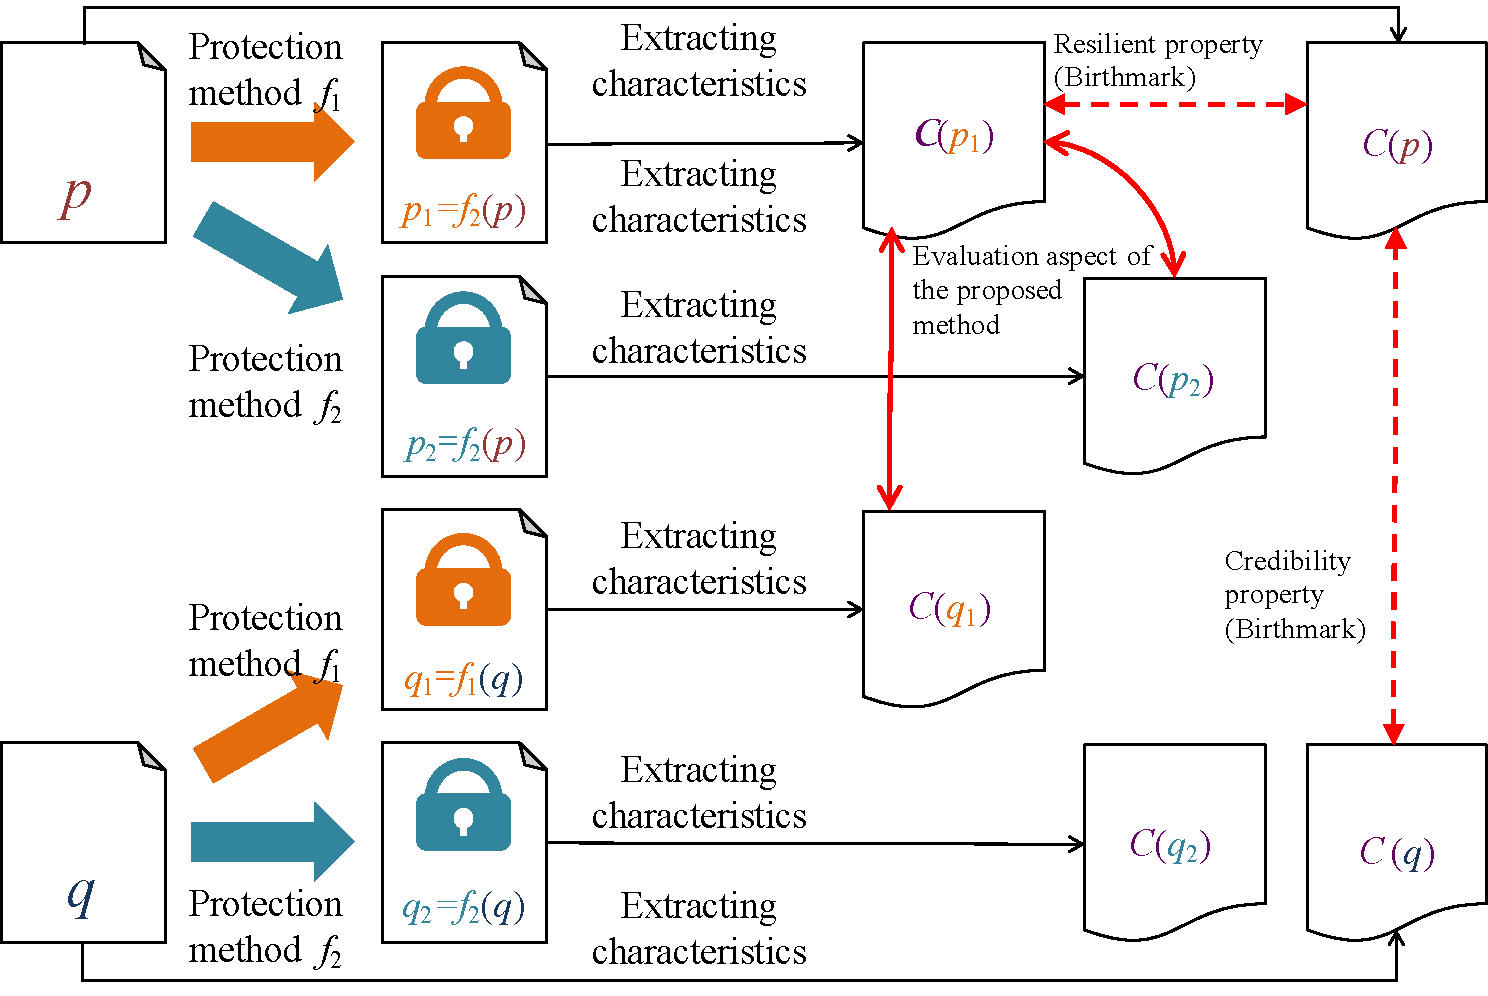
\includegraphics[width=0.49\textwidth]{images/key_idea}
  \caption{Key idea of the proposed method}\label{fig:keyidea}
\end{figure}

The birthmark methods have been proposed, which use characteristics of
the program\cite{tamada05ieice}.  Birthmark method originally computes
similarities between the programs with the extracted native
characteristics in order to detect pirated programs.
%
The process of our method is ported from birthmark methods, which is
to extract characteristics from the program, and to compare them.
However, extracting characteristics are absolutely different.  The
birthmark methods focus on the characteristics of the program.  Our
method focuses on the characteristics of the protection method.

On the other hands, Kanzaki et al. proposed the method to measure the
stealthiness of the program\cite{kanzaki14ipsj}. The method extracts
$n$-gram from the opcodes of the given program, and computes
artificiality by the probability from the corpus.  The artificiality
means how {\em natural} opcode sequences are in the target program.
Kanzaki et al. assume that a compiler generates natural opcode
sequences.  Generally, protection methods alter the opcode sequence by
their algorithm.  Then, the protected program may have unnatural
opcode sequences.  If a protection method have {\em natural} opcode
sequences, the algorithm of the method is stealthy.

We focus on the method to compute artificiality, and assume that
protected program have a certain characteristics of the protection
algorithm.  Then, we tackle to identify the protection method of the
program by the extracted characteristics.

Figure \ref{fig:keyidea} shows key idea of the proposed method.  In
the figure \ref{fig:keyidea}, we aquire obfuscatd program $p_1$ and
$p_2$ from original program $p$ by certain obfuscation algorithm $f_1$
and $f_2$ ($p_1 = f_1(p), p_2 = f_2(p)$).  Then, using characteristics
extraction function $\mathcal{C}$, we extract cetain characteristics
$\birth{p}$, $\birth{p_1}$, and $\birth{p_2}$ from $p$, $p_1$, and
$p_2$.

The evaluation aspects of the birthmark method are resilient property
and credibility property.  To evaluate resilient property compare
$\birth{p}$ and $\birth{p_1}$, then high score shows $p_1$ and $p$ are
copy relation.  Also, credibility property compare $\birth{p}$ and
$\birth{q}$, then, low score shows $p$ and $q$ are independently
developed.

The evaluation aspect of the proposed method is $\birth{p_1}$ and
$\birth{p_2}$, and $\birth{p_1}$ and $\birth{q_1}$.  Low score between
former relation ($\birth{p_1}$ and $\birth{p_2}$) shows different
protection methods were applied.  Also, high score between latter
relation ($\birth{p_1}$ and $\birth{q_1}$) shows same protection
method was applied.

% Base mark that is to distinguish others programs by characteristic in
% program is proposed\cite{tamada05ieice}.  Base mark is technique that
% is to find plagiarism by comparing characteristic with ones that
% program have originally.  For difference purpose from this research,
% it can not apply the base mark as it is, but it can expect the advance
% method of base mark as standard way of comparison.
% 
% Kanzaki's propose method that is to evaluate unnatural of
% program\cite{kanzaki14ipsj}.  This program is to expect n-gram from
% opcode in program and to evaluate unnatural by requiring generative
% probability.  For example, Matuda's evaluate difficult discovery of
% method of protection by comparing unnatural of fragment of
% code\cite{matsuda15ipsj}.
% 
% We assume that method of protection have a proper characteristic by
% forcing on this method.  Thus, for proper characteristic, we try to
% identify how method of protection are used.  If method of protection
% can be identified, specializing method of attack for and attack for
% the method of protection understanding to method of protection are
% possible.  Conversely, if method of protection can not be identified,
% the key of attack can not be taken and attack is difficult.

% It show a schematic diagram of method of protection at
% Figure\ref{fig:keyidea}.  Process method and base mark are same as
% processing that is to extract characteristic from protected program.
% On the other hand, evaluation point are different.
%%%% 
% %式が出るので後
%%%% 
% In Figure\ref{fig:keyidea}, protected program $p_1=f_1(p)$,
% $p_2=f_2(p)$ are gotten by any methods of protection $f_1$ と $f_2$
% with program $p$.
%%% 
% So, any characteristics $\birth{p_1}, \birth{p_1}, and \birth{p_2}$
% are gotten from $p, p_1, p_2$ , for using the feature extraction
% function$\mathcal{C}$.
%%% 
% The interest in base mark technology is part of showing a arrow by a
% dotted line in Figure\ref{fig:keyidea}.  As a result, we evaluate
% that how do $\birth{p}$, $\birth{p_1}, and \birth{p_2}$ look like?,
% and how do $\birth{p}$ and $\birth{q}$ look difference?
%%% 
% The interest in proposed method is part of showing a arrow by a
% solid line in Figure\ref{fig:keyidea}.  That is to say, we compare
% that how do protected same programs by different method look
% difference ($\birth{p_1}$と$\birth{p_2}$)? and how do protected
% different programs by same method look like?

\subsection{Characteristics of the Proposed Method}

To implement the proposed method, almost birthmark methods would fail
to identify the protection method.  Because, if we apply a certain
protection method $f_1$ to different programs $p$ and $q$, birthmark
method expects $\birth{p} \neq \birth{q}$.  However, the proposed
method expects $\birth{p_1} \approx \birth{q_1}$.

We focus on the artificiality evaluation method by Kanzaki et al. to
the proposed method.  A certain protection method inserts ridiculous
opcode sequence into never executed block.  Another certain protection
method change natural opcode sequence to unnatural one.  Such unnatual
opcode sequence might be characteristics of the protection method.

Originally, Kanzaki et al. computed the artificiality by probability.
Ohtaki et al. ported Kanzaki's method for object oriented language,
such as Java\cite{gekka14scis}.  The method uses perplexity metric
instead of Kanzaki's probability for computing the artificiality.  The
perplexity metric shows complexity of the natural language.  Low
perplexity means that next word is easy to expect.

On the other hand, a certain protection method duplicates original
natural opcode sequence.  Such duplicated sequence is still natural.
Therefore, we also focus on the frequencies of the $n$-gram.

Then, we employ the perplexity metric and frequency of the $n$-gram as
the characteristics of the protection method.

% Although Extracting characteristic is like base mark in method, it do
% not carry out as expected to itself.
% %式が出るので後
% 
% Because, in protected different program $p$ and $q$ by same method
% $f_1$, as base mark is that program itself is to difference, we expect
% result as difference($\birth{p_1} \neq\birth{q_1}$).  However, as
% proposed method is to take the characteristic in method of protection
% itself, we expect result as same($\birth{p_1} \approx \birth{q_1}$).
% 
% Therefore, we observe Kanzaki's propose method that is to evaluate
% unnatural of program\cite{kanzaki14ipsj}
% 
% This method is to use the rare in $n$-gram of opcode.  In method of
% protection, the case is absolutely to insert the sequence of orders in
% place that is not carried out impossibility, and other case is to
% rearrange rare order as understanding in original order is difficult.
% 
% Thus, we can judgment whether rare order is true or false as showing
% rarity.  it is to say that these rare order is characteristic in
% method of protection.  creation probability use the
% perplexity\cite{gekka14scis}.  Perplexity is known average branch and
% ais index that express complexity as language.  It is express that the
% more little this value is,the more next coming language is predicted.
% As a result, it is say that the more little the value is, the more
% natural value is.
% 
% On the other hand, in the method of protection, the case is that the
% compiler outputted original orders with repeated.
% 
% As The original order is difference with use frequency, it is not to
% say the rare.  Thus, the only creation probability is not able to
% observe the characteristic in method of protection.  Therefor, we
% observe the frequency in $n$-gram.
% 
% In the above, we extract order in $n$-gram from program, and are
% characteristic in method of protection with the rare ( perplexity )
% and frequency.
%

\section{Experimental evaluation}
\subsection{Overview}


そこで、Javaを対象とした難読化ツールを用い
て、実際にjarファイル$p, q, r$を難読化する。この難読化手法が$f_n$に相
当する。そして、難読化前後のjarファイルから特徴$\birth{p}, \birth{q},
\birth{r}, ..., \birth{p_n}, \birth{q_n}, \birth{r_n}$を抽出する。そし
て、得られた特徴をグラフにして、互いに比較する。

抽出する特徴は、第\ref{sect:artificiality}節で述べたようにオペコードの
$n$-gramを基本とし、そのパープレキシティと頻度を用いて比較を行う。

パープレキシティを導出するためにコーパスの構築が必要である。そのため、
The Apache Software Foundation\footnote{\url{http://www.apache.org/}}
で配布されているjarファイル 3,786 個を収集した。jarファイル内の総クラ
ス数は 660,465、総メソッド数は 4,272,567 である。

Some characteristic in method of protection have become clear by
preliminary experiment.  This purpose is how to decide the method of
protection from extracted characteristic.  As extracting
characteristic is based on n-gram of opcode such as chapter three,
verse 2, we compare its with perplexity and frequency.

we conducted a preliminary study to investigate the following
questions.  RQ1: What kind of characteristic in method of obfuscation?

RQ2-1:Is the characteristic effective measure for unknown product?

RQ2-2:Is the characteristic effective measure for unknown obfuscation?

\begin{table}[t]
  \centering
  \footnotesize{
    \caption{利用したJarファイル一覧}\label{table:jars}
  \begin{tabular}{l|r||l|r||l|r}
    Product & Version & Product & Version & Products & Version \\ \hline
    ASM       & 3.3.1 & FakeHack  & 1.0 &JCalendar & 1.3.3   \\
    Jhstop    & 0.0.1 & Jwhich    & 1.0   & Robocode-setup & 1.6.0.1 
  \end{tabular}
  \caption{利用した難読化ツール}\label{table:tools}
  \begin{tabular}{ll|l}
      Tools & Abbr. & Overview \\ \hline
      Allatori Java Obfuscator & ALL & 商用の難読化ツール \\ \hline
      ProGurad                 & PG & OSSの難読化ツール \\ \hline
      Sandmark                 & & 研究用の難読化ツール \\
      \hspace{0.2cm} Duplication registers & DR & 代入を重複させる。\\
      \hspace{0.2cm} Merge local integers & MLI & 2つのint変数をlongに収める。\\
      \hspace{0.2cm} Irreducibility       & IRR & 制御フローを複雑にする。\\
  \end{tabular}}
\end{table}

\subsection{analysis in n-gram}

In this purpose, we analyzed order in n-gram by referring to frequency
and perplexity in each method of obfuscation.  In the analysis result,
It see different order before and after protection in method of
obfuscation.

As a result, we analyze the RQ1.

Also, we understand that added order is high value of perplexity and
rare order.  For these data, added order As characteristic in method
of obfuscation is added order by these datas, the characteristic are
reported TABLE\ref{table:features}.



\begin{table}[t]
  \centering
  \footnotesize{
    \caption{ツールごとの特徴}\label{table:features}
  \begin{tabular}{l|l}
    ツール              & 特徴 \\ \hline
    ALL & オリジナルの命令列を\texttt{swap}命令で入れ替える \\
    PG  & オリジナルと変化なし \\
    DR  & \texttt{istore}命令を2回続けて実行する \\
    MLI & \texttt{dup2x2 lxor}を連続して実行する \\
    IRR & \texttt{nop}命令がある \\
  \end{tabular}}
\end{table}


\subsection{identifying method of obfuscation in known}

In this purpose, unknown product are obfuscated by using the tools in
TABLE\ref{table:features}, after we identify how method of obfuscation
are used.

As a result, we analyze the RQ2-1.

Not appearing n-gram are researched by n-gram that is before applied
obfuscation.  In the result, n-gram of high frequency in five is
reported TABLE\ref{table:junit}.  In showing the
TABLE\ref{table:junit}, the order are called high value in perplexity
such as dup2X2 lxor.  As the order is characteristic, we compare it
with characteristic in five tool ( TABLE\ref{table:junit} ).  As a
result, characteristic in applied method of obfuscation correspond
with characteristic in method of MLI.

\begin{table}[t]
  \centering
  \footnotesize{
    \caption{JUnit (5-gram)の命令列}\label{table:junit}
  \begin{tabular}{l|r|r}
    命令列 & 頻度 & PPL\\ \hline
 %   \multicolumn{1}{p{1cm}}{ORI} & 
 %   \multicolumn{1}{p{1cm}}{ALL} & 
 %   \multicolumn{1}{p{1cm}}{DR} & 
 %   \multicolumn{1}{p{1cm}}{IRR} & 
 %   \multicolumn{1}{p{1cm}}{MLI} & 
 %   \multicolumn{1}{p{1cm}}{PG} & 
 %   \multicolumn{1}{p{1cm}}{PPL} \\ \hline
    \texttt{dup2x2 lxor lconst\_1 lneg bipush}   & 16 & 11.30E+05 \\
    \texttt{lload dup2x2 lxor lconst\_1 lneg}    & 16 &   5.37E+05 \\
    \texttt{bipush lushr land lxor lstore}       &  9 &   0.52E+05 \\
    \texttt{lconst\_1 leng bipush lushr land}    &  9 &   0.96E+05 \\
    \texttt{lneg bipush lushr land lxor}         &  9 &  1.37E+05 \\
  \end{tabular}}
\end{table}

\subsection{identifying method of obfuscation in unknown}

In this purpose, known products are obfuscated by using the unknown
method of obfuscation, after we identify how method of obfuscation are
used.

As a result, we analyze the RQ2-2.

Not appearing n-gram are researched by n-gram that is before applied
obfuscation.  In the result, n-gram of high frequency in five is
reported TABLE\ref{table:jhstop}.  In showing the
TABLE\ref{table:jhstop}, the order that is high value in perplexity
are called dup and imul orders in continuous.  As the order is
characteristic, we compare it with characteristic in five tool (
TABLE\ref{table:jhstop} ).  As a result, characteristic in unknown
method of obfuscation do not correspond with characteristic in
analyzed method.

In the next, as difference product are obfuscated unknown method of
obfuscation, we compare the each characteristic.  As a result, as the
same characteristic are identified, we understand that unknown method
of product is method of SOP.


\begin{table}[t]
  \centering
  \footnotesize{
    \caption{Jhstop (5-gram)の命令列}\label{table:jhstop}
  \begin{tabular}{l|r|r}
   命令列 & 頻度 & PPL\\ \hline
 %   \multicolumn{1}{p{1cm}}{ORI} & 
 %   \multicolumn{1}{p{1cm}}{ALL} & 
 %   \multicolumn{1}{p{1cm}}{DR} & 
 %   \multicolumn{1}{p{1cm}}{IRR} & 
 %   \multicolumn{1}{p{1cm}}{MLI} & 
 %   \multicolumn{1}{p{1cm}}{PG} & 
 %   \multicolumn{1}{p{1cm}}{PPL} \\ \hline  
    \texttt{irem iconst\_0 if\_icmpne aload getfield} & 15 &   0.15E+05 \\
    \texttt{dup dup dup imul imul}                    & 14 &  42.40E+05 \\
    \texttt{dup dup imul imul isub}                   & 14 &   8.74E+05 \\
    \texttt{dup imul imul isub iconst\_3}             & 14 &   3.49E+05 \\
    \texttt{iload dup dup dup imul}                   & 14 & 101.00E+05 \\
    \end{tabular}}
\end{table}


\section{Conclusion}
In this paper, we took the identification of method of protection by
watching the unnatural evaluation.  The actual program was applied
method of protection and extracted characteristic to base on frequency
and perplexity to order line of n-gram.  In this evaluation
experiment, the identification of known obfuscation is easy and the
identification of unknown obfuscation is difficult.  This solution
plan is to increase the characteristic of method of obfuscation.  it
can respond to method of unknown obfuscation by increasing
characteristic.

% \section*{Acknowledgment}

\bibliographystyle{IEEEtran}

\bibliography{icis2016_sagisaka}

\end{document}


